% --------------------------------------------------------------------------
% Template for WASPAA-2019 paper; to be used with:
%          waspaa17.sty  - WASPAA 2019 LaTeX style file, and
%          IEEEbib.bst - IEEE bibliography style file.
%
% --------------------------------------------------------------------------

\documentclass{article}
\usepackage{waspaa17,amsmath,amssymb,graphicx,url,times}
%\usepackage{waspaa17,amssymb,amsmath,graphicx,times,url}
\usepackage{color}
\usepackage{tabularx,booktabs,colortbl}
\usepackage{hyperref,subfig}
% Example definitions.
% --------------------
\def\defeqn{\stackrel{\triangle}{=}}
\newcommand{\symvec}[1]{{\mbox{\boldmath $#1$}}}
\newcommand{\symmat}[1]{{\mbox{\boldmath $#1$}}}

% Title.
% --------------------
\title{Estimation of Guitar String, fret and plucking position using a physical model and no training data}
% Improved phyiscial models for faster and better estimation of guitar string, fret and plucking position.
%% Single addresses (uncomment and modify for single-address case).
%% --------------------
%\name{Author(s) Name(s)\thanks{Thanks to XYZ agency for funding.}}
%\address{Author Affiliation(s)}
%%
%% For example:
%% ------------
%%\address{School\\
%%       Department\\
%%       Address}
% ---------------
\name{Jacob~M\o ller Hjerrild, Silvin Willemsen and~Mads~Gr\ae sb\o ll~Christensen}%\thanks{Thanks to XYZ agency for funding.}}
\address{Audio Analysis Lab, CREATE, Aalborg University, Denmark\\
   \texttt{\{jmhh, sil, mgc\}@create.aau.dk}}
%


\begin{document}

\ninept
\maketitle

\begin{sloppy}

\begin{abstract}
  In this paper a method for analyzing guitar performances is proposed. This method extracts the activated string and fret as well as the plucking position, and it is purely based on a physical model of string excitation and vibration, hence it does not require any training data which makes it fast and effective. Since it operates on a 40 ms segment-by-segment basis it is suitable for real-time estimation...
\end{abstract}
%
\begin{keywords}
 Physical Modeling, Statistical Signal Processing, Parametric Pitch Estimation, Music Information Retrieval\vspace{-.8mm}
 \end{keywords}
%
\section{Introduction}
\label{sec:intro}
%
Recordings of music performances can be analyzed for various reasons, such as extracting stylistic details, artist recognition or detailed transcription of individual instruments, which can provide means for increasing usability of music learning technologies...

As shown in [REFERENCES], the inharmonicity of a guitar signal can be utilised to accurately estimate string, fret and plucking position. Inharmonicity in instruments strings arises because of the presence of stiffness in the strings. Therefore, the partial amplitudes are not located as perfect multiples of the fundamental frequency, but are rather stretched towards the higher end.
% Specifically, the activated string and fret as
% well as the location of the plucking event along the guitar string are
% extracted from guitar signal recordings

Furthermore, nearly all literature on the topic of inharmonicity, ignores or assumes part of the physics. This includes, but is not limited to, the contribution of the string wrapping and the contribution of the initial string displacement to the total inharmonicity. In this paper we attempt to accurately model these two 'left out' parts of the physics of the string and observe whether this ultimately makes a difference in our estimation.

% In this paper, we discuss how to obtain such a model based only on physical string parameters, such that we can exclude the requirement for training data, based on recordings.

\section{Problem Formulation}
The overall problem in this paper is the estimation of the guitar string, fret and plucking position without requiring any audio for training a model. The feature set is based on~\cite{hjerrild::icassp19} where pitch $\omega_0$ and inharmonicity $B$ is extracted with a parametric pitch estimator.  Instead of training a model from audio recordings, we propose a simulated model of guitar string vibrations based on physical properties such as dimensions and materials. Figure~\ref{fig:guitar_overview} gives an overview of the guitar, where 
\begin{figure}[h!]\
  \centering
  \centerline{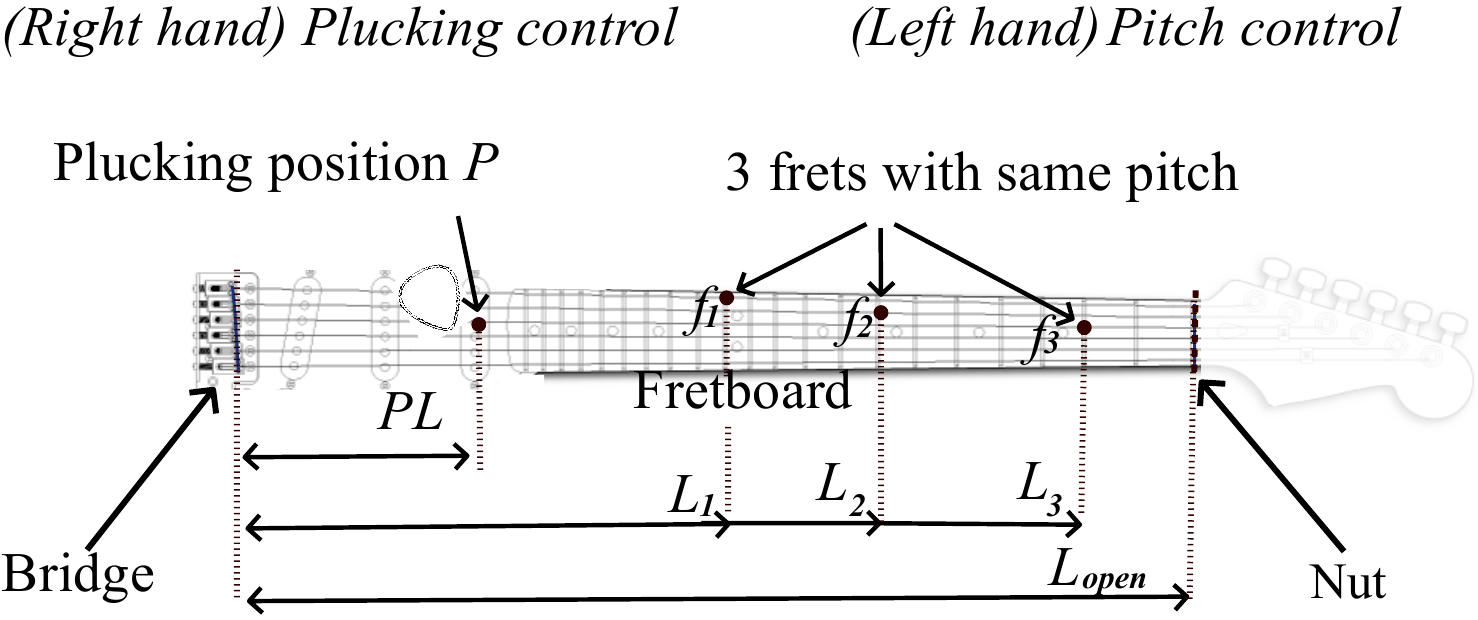
\includegraphics[width=1\columnwidth]{img/fender_drawing4.png}}
  \caption{The plucking position is controlled by the right hand while the left hand controls pitch using the fretboard. Similar pitch is produced in various positions. Source: Adapted from~\cite{phillips}.
  }\label{fig:guitar_overview}\vspace{-2mm}
\end{figure}
%
the right hand controls plucking position and the left hand controls pitch by using the fretboard. One pitch is produced in various positions and each string and fret combination is defined as one class, such that we have a set of $K$ mutually exclusive classes. 
%
%
%
% 
As demonstrated in~\cite{hjerrild::icassp19} a maximum likelihood classifier with a physically meaningful feature set consisting of pitch $\omega_0$ and inharmonicity $B$ can be utilized for distinguishing between string and fret combinations. 
Since the string is inharmonic the $m$th instantaneous frequency $\psi(\omega_0,B)$ is defined by the piano string model derived in~\cite{fletcher:piano_model} as 
%
\begin{equation}\label{eq:pianoModel}
  \psi_m(\omega_0,B) = m \omega_0 \sqrt{1+B m^2} \quad [\text{s}^{-1}], 
\end{equation}
where fundamental frequency $\omega_0$ and inharmonicity coefficient $B$ can be estimated without detailed knowledge of the physics that defines the inharmonicity~\cite{ hjerrild::icassp19,abesser:automatic_string_detection_ml, barbancho:inharmonicity_tablature,michelson2018_aes}. 
However, modelling all classes on the guitar requires training data captured from each class. For 6 strings and 12 frets that is $K=72$  classes. Although~\cite{hjerrild::icassp19,barbancho:inharmonicity_tablature} shows that a fast training procedure requires only training data captured from one fret per string. There are three main challenges associated with such a a fast training procedure,%, which requires some work from the user. 
\begin{itemize}
    \item There is no information of class dependent distributions in the observed feature space, i.e. covariance structures. Except from the 6 classes represented in the training set.
    \item With only a few observations (i.e. 10 per string~\cite{hjerrild::icassp19}), it is impossible to conclude anything significant on the covariance structure of each class.
    \item Although training is relatively fast, it is required for every time for every different set of guitar strings.
%    \item  Can we eliminate the training procedure that requires recordings ?
%    \item  Can we extract the inharmonicity with higher precision based on the physical model of plucking ?
\end{itemize}
Can we eliminate the training procedure that requires the user to provide recordings and at the same time obtain a detailed and class dependent distribution in the feature space? To overcome these problems, we will build a model from string material properties and dimensions. Detailed information of such properties are generally available on string packets.

%
%
%
%
%
%With detailed knowledge of the inharmonicity it is in fact possible to obtain a model for all frets on a string from one such model. In example, given the parameters $B_s( f_1 )$ and $\omega_{0,s}( f_1 )$ of the $s$th vibrating string for a given fret $f_1$, the corresponding parameter can be computed for any other fret $f_2$, using the inharmonicity model based on knowledge of the equal tempered scale as derived in~\cite{barbancho:inharmonicity_tablature}
%\begin{equation}
%    \widehat{B}_s( f_2 ) =  \widehat{B}_s( f_1 ) \: 2^{ \frac{  f_2 - f_1 }{ 6 }} = \frac{ \pi^3 E_s d_s^4 }{ 64 T_s L^2_{s}(f_2) } \quad [\cdot],
%\end{equation}
%where $E, d, T$ are the elastic Modulus, diameter and tension of the core which are considered constants and $L(f_2)$  is the length from the bridge to the given fret $f_2$.
%For the pitch estimates we have that the relation is
%\begin{equation}\label{eq:omega0_fast}
%  \widehat{\omega}_{0,s}( f_2 ) =  \widehat{\omega}_{0,s}( f_1 ) 2^{\frac{f_2-f_1}{12}} \quad [s^{-1}].
%\end{equation}
%
%
%
%
%
%
%
%
% 
\newcommand{\ts}{\textsuperscript}

\newcommand{\fret}{f}


\newcommand{\veca}{\mathbf a}
\newcommand{\vecx}{\mathbf x}
\newcommand{\vecs}{\mathbf s}
\newcommand{\vecv}{\mathbf v}
\newcommand{\matV}{\mathbf V}
\newcommand{\vecz}{\mathbf z}
\newcommand{\vecX}{\mathbf X}
\newcommand{\mtrxsigma}{\mathbf{\Sigma}}
\newcommand{\argmax}[1]{\underset{#1}{\operatorname{argmax}}\;}
\newcommand{\argmin}[1]{\underset{#1}{\operatorname{argmin}}\;}


\newcommand{\colvec}[4]{ \begin{bmatrix} #1 \\ #2 \\ #3 \\ #4\end{bmatrix} }
\newcommand{\rowvec}[4]{ \begin{bmatrix} #1 & #2 & #3 & #4 \end{bmatrix} }



 % ---- Make typing equations easier -------------\c
\newcommand{\ahat}{\hat{\alpha}}
\newcommand{\C}{\boldsymbol{\zeta}}
\newcommand{\Like}{\mathcal{L}}
\newcommand{\Piz}{\boldsymbol\Pi_{Z}}
\newcommand{\Thetaparam}{\boldsymbol\Theta}
\newcommand{\HATThetaparam}{\hat{\boldsymbol\Theta}}
\newcommand{\thetaparam}{\boldsymbol\theta}
\newcommand{\thetahat}{\hat{\boldsymbol\theta}}
\newcommand{\limN}{\lim_{N\to\infty}}
\newcommand{\var}{\sigma^2}
\newcommand{\varhat}{\hat{\sigma}^2}
\newcommand{\z}{\mathbf{z}}
\newcommand{\ehat}{\hat{\mathbf{e}}}
\newcommand{\matZ}{\mathbf{Z}}
\newcommand{\matS}{\mathbf{S}}
\newcommand{\Z}{\mathbf{Z}}
\newcommand{\x}{\mathbf{x}}
\newcommand{\s}{\mathbf{s}}
\newcommand{\shat}{\mathbf{\hat{s}}}
\newcommand{\I}{\mathbf{I}}
\newcommand{\pz}{p(\mathbf{z})}
\newcommand{\pwz}{p(\omega|\mathbf{z})}
\newcommand{\Pwz}{P(\omega|\mathbf{z})}
\newcommand{\Pw}{P(\omega)}
\newcommand{\pwg}{p(\mathbf{w}|\gamma)}
\newcommand{\pwgk}{p(\mathbf{w}|\gamma_k)}
\newcommand{\Pzw}{P(\mathbf{z}|\omega)}
\newcommand{\w}{\omega}
\newcommand{\vecmu}{\text{\boldmath$\mu$}}
\newcommand{\what}{\hat\omega}
\newcommand{\Cost}{C(\hat\omega_i|\omega)}
\newcommand{\Risk}{R(\hat\omega_i|\z)}
\newcommand{\E}{\mathrm{E}} 
 % -----------------------------------------------

\newcommand{\vecr}{\mathbf r}
% section describing the guitar tuner harmonic summation
\newcommand{\NFFT}{\texttt{NFFT}}
\newcommand{\N}{\texttt{N}}
\newcommand{\dur}{\texttt{dur}}
\newcommand{\vecf}{\mathbf f}
\newcommand\numberthis{\addtocounter{equation}{1}\tag{\theequation}}
\newcommand{\HL}{\bm{HL}}
\newcommand{\PSNR}{\textit{PSNR}}
\newcommand{\SNR}{\textit{SNR}}
\newcommand{\PSNRvec}{\mathbf{PSNR}}
\newcommand{\SNRvec}{\mathbf{SNR}}
\newcommand{\RMSE}{\textit{RMSE}}
%% -----------------------------------------------------
\newcommand{\vectheta}{\text{\boldmath$\theta$}}
\newcommand{\vecphi}{\text{\boldmath$\phi$}}
\newcommand{\vecPhi}{\text{\boldmath$\Phi$}}
\newcommand{\vecalpha}{\text{\boldmath$\alpha$}}
\newcommand{\vecalphahat}{\text{\boldmath${\widehat\alpha}$}}

\newcommand{\norm}[1]{\left\lVert#1\right\rVert}

%
%\newcommand{\ts}{\textsuperscript}

%\newcommand{\veca}{\mathbf a}
% \newcommand{\vecX}{\mathbf X}
% \newcommand{\vecmu}{\mathbf{\mu}}
%\newcommand{\mtrxsigma}{\mathbf{\Sigma}}
% \newcommand{\argmax}[1]{\underset{#1}{\operatorname{arg}\,\operatorname{max}}\;}
% \newcommand{\argmin}[1]{\underset{#1}{\operatorname{arg}\,\operatorname{min}}\;}


% \newcommand{\colvec}[4]{ \begin{bmatrix} #1 \\ #2 \\ #3 \\ #4\end{bmatrix} }
% \newcommand{\rowvec}[4]{ \begin{bmatrix} #1 & #2 & #3 & #4 \end{bmatrix} }
 \newcommand{\symvec}[1]{{\mbox{\boldmath $#1$}}}
 \newcommand{\symmat}[1]{{\mbox{\boldmath $#1$}}}
\section{signal model}
The signal model is derived from the string vibrations, thus we start by describing the activation from the guitar pick. 
%
The string has an initial deflection $\delta$ at the plucking position, which is at the $P$th fraction of its length $(0<PL<L)$, where $L$ is the length of the vibrating string. At release the displacement $y$ is defined by the 1D wave equation: %
%\begin{equation}
$\frac{\partial^2y}{\partial t^2} = c^2\frac{\partial^2y}{\partial l^2}$,
%\end{equation}
%
where $c$ is the transverse wave speed. Assuming that the string is pinned at $l=0$ and $l=L$, its general solution can be written as~\cite{fletcher:physics_of_musical_instruments}:
%
\begin{equation}\label{eq:modalSum}
    y(l,t) = \sum_m C_m\sin(\omega_mt+\phi_m)\sin\kappa_ml,
\end{equation}
%
where $C_m$ is the amplitude of the $m$th mode, $\omega$ is frequency and $\kappa_m = \omega_m / c$. Assuming the initial displacement to be triangular and no initial velocity $\frac{\partial y}{\partial t} = 0, \, \forall\, l$, the $m$th amplitude $C_m$ is defined by the Fourier sine series~\cite{donkin:acoustics,fletcher:principles_of_vibration_and_sound}:
\begin{equation}
    C_m = \frac{2\delta}{m^2\pi^2P(1-P)}\sin(m\pi P), \quad [\cdot],
\end{equation}
which expresses that the spectral envelope is sinusoidally shaped, dependent on the plucking position $P$ with a scale of $m^{-2}$ for the $m$th mode.
%
\noindent
On the guitar we assume that a pickup is measuring the displacement $y(l,t)$ close to the string at location $l\!\!=\!\!\lambda$. At the discrete time instance $n$ the observed signal $x(n)$ is being sampled, i.e.,
\begin{equation}
     x(n)  \vert_{l=\lambda} \propto y(\lambda, t),
\end{equation}   
where $x(n)$ is the guitar signal recorded with the pickup at $\lambda$. We parametrize $x(n)$ with an inharmonic signal model as proposed in~\cite{hjerrild::icassp19}. 
%
 At time instance $n$, the observed signal vector $\vecx \in \mathbb{C}^N$ is represented as $\vecx = [x(0) \, x(1) \, \cdots \, x(N-1)]^T$, with $T$ denoting the transpose. %Do we need this?
%A complex signal can ease both notation and computational complexity and a real-valued signal is converted to complex by using the Hilbert transform~\cite{LawrenceMarple1999}. 
The $n$th entry of $\vecx$ is modeled as an inharmonic sinusoidal part and a noise part i.e.,  
\begin{equation}\label{eq:sigmod1}
  x(n)\! =  \!\sum\limits_{m=1}^{M}\!\! \alpha_{m} \exp\big({j\psi_m(\omega_0,B) n}\big)+v(n), 
  %x(n)\! = \!s(n)\!+\!v(n)\!= \!\sum\limits_{m=1}^{M} \alpha_{m} e^{j(m\omega_0 \sqrt{1+B m^2}) n}+v(n), 
\end{equation}
where $\omega_0$ is the fundamental frequency, $M$ is the number of partials, $\alpha_{m}$ is the complex amplitude of the $m$th partial, $v(n)$ is noise and the instantaneous frequency  $\psi_m(\omega_0,B)$ is derived in~\cite{fletcher:piano_model} as
\begin{equation}
  \psi_m(\omega_0,B) = m \omega_0 \sqrt{1+B m^2}. 
\end{equation}
For ease of notation, we denote it as $\psi_m$ although it is a function of $\omega_0$ and $B$. The model order $M$ can be estimated~\cite{nielsen2017fast,multipitch}, while for the string model, initialized by the triangular shape in~\eqref{eq:string_initialization} we assume a high $M$ at the onset event. In vector-matrix notation the observed signal is modeled as
\begin{equation}\label{eq:xZa}
  \vecx = \matZ \vecalpha + \vecv,
\end{equation} 
where the complex sinusoidal matrix $\matZ \in \mathbb{C}^{N\times M}$ is given by
\begin{align}
  \matZ =& \left[ \vecz(\psi_1) \: \vecz(\psi_2) \: \cdots \: \vecz(\psi_M)\right], \\
  \vecz(\psi_m) =& \left[ 1 \: e^{j\psi_m} \: e^{j\psi_m2} \: \cdots \: e^{j\psi_m(N-1)} \right]^{T},
\end{align}
where $\vecalpha = [\alpha_1 \: \cdots \: \alpha_M]^T$ is a vector containing complex amplitudes and $\vecv = [v(0) \: v(1) \: v(N-1)]^T$ contains all noise terms. We denote the unknown and deterministic parameters with $\vectheta$, i.e.
\begin{equation}\label{eq:theta_parameters}
  \vectheta = \{\omega_0, B, \vecalpha\}.
\end{equation}
The amplitudes $\vecalpha$ can be estimated with the least squares, while the other parameters $\omega_0$ and $B$ are non-linear. 
The inharmonic pitch and inharmonicity coefficient estimates $\{\widehat\omega_0, \widehat B \} $ are sufficient for classification of string and fret~\cite{barbancho:inharmonicity_tablature,michelson2018_aes} and the estimated amplitude vector $\vecalphahat$ is used for estimation of the plucking position $\widehat{P}$.
\section{Inharmonic string model} \label{sec:string_model}

% \subsection{Intrinsic and deflection-caused inharmonicity}
As opposed to the ideal string, the frequencies in the inharmonic string model are calculated using \eqref{eq:pianoModel}. The authors of \cite{coltShank} state that string inharmonicity arises from two sources: the intrinsic inharmonicity due to the $\textit{stiffness}$ of the string and inharmonicity due to $\textit{stretching}$ of the string during the initial pluck. Rossing in \cite{rossing:science_of_string_instruments} quantifies the effect of both by introducing a factor $K$:
\begin{align}
    K = \frac {\pi^3 E d_\text{c}^2}{16 T_0 L^2}, \quad [\text{m}^{-2}],
\end{align}
with string-core diameter $d_\text{c}$, string-tension $T_0$, string-length (nut to bridge) $L$ and Young's Modulus $E$ of the string material defined in \eqref{eq:tensile_stress}. The intrinsic inharmonicity is defined as
\begin{align}\label{eq:intrinsicInharmonicity}
    B_\text{i} = \frac {K}{4} d_\text{c}^2  \quad [\cdot],
\end{align}
and the inharmonicity due to plucking with maximum transverse displacement $\delta$ (pluck amplitude) is  
\begin{align}\label{eq:displacementInharmonicity}
    B_\delta = \frac {3K}{8} \delta^2 \quad [\cdot],
\end{align}
if $P=0.5$, i.e. if the string is plucked at the center.
%This pitch shift is responsible for the initial twang (\textbf{isn't this twang especially due to higher frequency content at the beginning of the pluck} of the string and dies down rapidly after the pluck. It is assumed
%
% According to~\cite{fletcher:piano_model} the $\textit{intrinsic string inharmonicity}$ $B_i$ is
%
% \begin{equation}
%     B_i = \frac{\pi^2 E A R_g^2}{T L^2}, \quad [\cdot],
% \end{equation}
% where the radius of gyration $R_g^2 = \frac{I}{A} = \frac{\pi}{4}\big(\frac{d_\text{c}}{2}\big)^4 \frac{1}{A}$ assuming a one-dimensional - not planar - radius of gyration
% %
% \begin{equation}\label{eq:intrinsicInharmonicity}
%     B_i =  \frac{\pi^3 E d_\text{c}^4}{64 T L^2} = \frac{\pi^2 E d_\text{c}^2}{64\rho_{\text{eff}} L^4 \omega_0^2}\quad [\cdot].
% \end{equation}
The total inharmonicity can then be defined as
\begin{equation}\label{eq:totalInharmonicity}
    B =  B_\text{i} + B_\delta =  \frac{\pi^3 E d_\text{c}^2(2d_\text{c}^2 + 3\delta^2)}{128 T_0 L^2}\quad [\cdot].
\end{equation}
It is expected that $d_\text{c}\ll\delta$, i.e. the initial displacement is likely to be more than an order of magnitude greater than the string diameter. Hence, the inharmonicity caused by the pluck dominates the intrinsic inharmonicity. However, this is only true immediately after the pluck, as the effect of $B_\delta$ is only predominant immediately after the pluck. Presumably, this is the reason why the literature on this topic has disregarded the initial displacement in the calculation of inharmonicity. As in our application, we solely use the first 40 ms of the plucked string sound, it is of utmost importance to include the effect that the initial displacement has on the total inharmonicity.

In the rest of this section, we will extend on the state of the art by providing more precise calculations for different aspects of the inharmonicity coefficient.

\subsection{Calculating pluck deflection at arbitrary pluck-position}
When calculating the inharmonicity due to plucking in \eqref{eq:displacementInharmonicity}, it is assumed that $P = 0.5$. Realistically, the plucking position will rarely, if not never, be in the middle of the string. We can calculate $\delta$ in \eqref{eq:displacementInharmonicity} from the transverse displacement at the $P$th fraction of the string-length $\delta_P$ where $P \neq 0.5$ utilising the change in string length due to plucking. This is calculated using
\begin{equation}\label{eq:changeLengthPluck}
    \Delta L_P = \sqrt{(LP)^2+{\delta_P}^2}+\sqrt{(L(1-P))^2+{\delta_P}^2} - L.
\end{equation}
This length extension can be used to calculate $\delta$ as if the string were plucked in the center. This will also retain the tension present in the string as $T_0$ and $\Delta L$ are proportional according to \eqref{eq:tensile_stress}. Setting $P = 0.5$, we can simplify \eqref{eq:changeLengthPluck} to
%
\begin{equation}\label{eq:changeLengthPluckHalf}
    \Delta L_{0.5} = 2\sqrt{(0.5L)^2 + \delta^2} - L.
\end{equation}
%
Replacing $\Delta L_{0.5}$ with the length extension $\Delta L_P$ calculated in \eqref{eq:changeLengthPluck} and solving \eqref{eq:changeLengthPluckHalf} for $\delta$ yields
\begin{equation}
    \delta = \frac{\sqrt{{\Delta L_P}^2+2L\Delta L_P}}{2},
\end{equation}
which can be used to calculate the inharmonicity due to plucking.
\subsection{Inharmonic pitch definitions for the wrapped string %Introducing the effect of wrapping
}

In the following we derive the model of pitch and inharmonicity by assuming that we know the string length, core and wrapping diameter,  material densities and fundamental frequencies. The inharmonicity is highly correlated with the core diameter $d_\text{c}$ and string inharmonicity has been an area of research for more than a century see i.e.,~\cite{rayleigh:sound}. For string designers, it is in general desired to lower the inharmonicity. For low-pitched strings it is not desired to simply increase the core diameter in order to lower the fundamental frequency as inharmonicity will increase by a power of 4 (as can be seen in \eqref{eq:intrinsicInharmonicity}). Therefore the strings are wrapped to add mass to the string to lower the pitch without affecting the inharmonicity by much. (BUT IT DOES A LITTLE: SEE SECTION INCLUDING $T_\text{c}$ AND $T_\text{w}$).

\noindent The mass per unit length $\mu$ of a wrapped string is defined by:

\begin{equation}
    \mu = \frac{\pi}{4}\Big(\rho_\text{c}d_\text{c}^2 + \rho_\text{w}\big[(2d_\text{w}+d_\text{c})^2-d_\text{c}^2\big]\Big), \quad [\text{kg}\cdot\text{m}],
\end{equation}
where $d_\text{c}$, $d_\text{w}$ are the core and wrapping diameters and $\rho_\text{c}$, $\rho_\text{w}$ are the densities of the core and wrapping respectively. When the string is single-cored ($d_\text{w} = 0$), and thus not wrapped, the second term becomes zero. Since the tension mainly acts on the core, the string can be considered a single cored string having the same mass per unit length $\mu$, but with the diameter of the core $d_\text{c}$ only. The effective density of this theoretical material is defined as~\cite{firth:string_design} (with $\frac{\pi}{4}$ removed)
\begin{equation}
    \rho_{\textup{eff}} = \rho_\text{c} + \rho_\text{w} \big[(1+2\frac{d_\text{w}}{d_\text{c}})^2-1\big], \quad [\text{kg}\cdot\text{m}^{-3}].
\end{equation}
This effective density can be used to calculate the pitch for the string, from the tension and length. The relation between the string length (nut-bridge) $L$, the tension $T$ and the pitch $\omega_0$ is:

\begin{equation}\label{eq:tension}
    T = \pi (L\omega_0)^2d_\text{c}^2\rho_{\textup{eff}} = \mu(2L\omega_0)^2, \quad [\text{N}],
\end{equation}
from which the equation for pitch can easily be derived:
\begin{equation}
    \omega_0 = \sqrt{\frac{T}{\mu}} \frac{1}{2L} \quad [\text{s}^{-1}],
\end{equation}
where the mass and length are being considered as constants. 
%
%
%
%
\subsection{Calculating Young's Modulus $E$ for wrapped strings}%Calculating strain length $\Delta L$ from material properties}
%
When the string is brought to pitch (tuned) it stretches according to its Young's modulus (or elastic modulus) $E$ which is defined as
%
\begin{equation}\label{eq:tensile_stress}
    E = \frac{\text{Tensile stress}}{\text{Strain}}
   %= \frac{T/A_\text{c}}{\Delta L/(L - \Delta L)} 
    = \frac{T/A_\text{c}}{\Delta L/(L - \Delta L)} \quad [\text{N}\cdot\text{m}^{-2}], 
\end{equation}
%
where $A_\text{c} = \pi d_\text{c}^2/4$ is the cross sectional area of the string-core and $\Delta L$ is the amount by which the string is stretched. The variables $E$, $A_\text{c}$ and $L$ are constants and $T$ and $\Delta L$ are proportional to each other. Important to note is that we use $L - \Delta L$ to describe the original string length before stretched to $L$.

The Young's modulus is a property defines for solid materials. Even though the string core and wrapping could be the same material, the wrapping is not solid! This means that when calculating the total inharmonicity using \eqref{eq:totalInharmonicity} for a wrapped string, the Young's modulus will be incorrect. In this section we will show a way to calculate an 'effective' Young's modulus $E_\text{eff}$ which can be used for calculating the inharmonicity. 

It requires high precision to measure $\Delta L$ in a guitar string. It is, however, possible to calculate it from material constants. For the core of the string we can rewrite~\eqref{eq:tensile_stress}, i.e.,
%
\begin{equation}\label{eq:deltaL}
    \Delta L= \frac{LT_\text{c}}{A_\text{c}E + T_\text{c}}, \quad  [\text{m}], 
\end{equation}
%
where $T_\text{c}$ is the tension contributed by the core. For single-cored strings $T_\text{c} = T$.
%
The effect of wrapping on the tension is small, though not neglegible. We can assume the wrapping to be a spring with spring constant~\cite{childs:mechanical_engineering}
%
\begin{equation}\label{eq:k_wrapping}
    k = \frac{Gd_\text{w}^4}{8ND^3}, \quad [\text{N}\cdot\text{m}^{-1}].
\end{equation}
%
Here, $G$ is the shear modulus of the wrapping material, $N = \frac{L - \Delta L}{d_\text{w}}$ is the number turns in the coil (assuming that for the untensioned string, every coil touches the previous and the next coil) and $D = d_\text{c}+d_\text{w}$ is the mean diameter of the spring~\cite{kemp:wound_and_unwound_strings}.
%
The length extension $\Delta L$ for a spring is
%
\begin{equation}\label{eq:deltaL_wrapping}
    \Delta L = \frac{T_\text{w}}{k}, \quad [\text{m}],
\end{equation}
%
where $T_\text{w}$ is the tension contributed by the wrapping. As in \eqref{eq:k_wrapping}, $k$ is dependent on $\Delta L$ (through variable $N$), we rewrite  \eqref{eq:deltaL_wrapping} to isolate $\Delta L$:
\begin{equation}\label{eq:deltaLwrappingIsolated}
    \Delta L = T_\text{w}\frac{8(\frac{L - \Delta L}{d_\text{w}})D^3}{Gd_\text{w}^4} = \frac{8T_\text{w}LD^3}{Gd_\text{w}^5 + 8T_\text{w}D^3} \quad [\text{m}].
\end{equation}
% We know the desired tension $T$ for all strings. However, we can not fill this into the above formulas because the  the core and wrapping have a very different contribution on the total tension. 
Furthermore, we know that the core and wrapping are part of the same string, meaning that they undergo the same length-extension $\Delta L$. We can thus set~\eqref{eq:deltaL} equal to~\eqref{eq:deltaLwrappingIsolated}, i.e., 
%
\begin{equation}
    \Delta L = \frac{LT_\text{c}}{A_\text{c}E + T_\text{c}} = \frac{8D^3LT_\text{w}}{Gd_\text{w}^5 + 8D^3T_\text{w}} \quad [\text{m}].
\end{equation}
%
As we know the desired tension $T$ through \eqref{eq:tension} and $T = T_\text{c} + T_\text{w}$, we can calculate the effect of the core and wrapping tensions:
%
\begin{equation}
    T_\text{c} = \frac{8A_\text{c}D^3ET}{Gd_\text{w}^5+8A_\text{c}D^3E}\text{ , } \newline
    T_\text{w} = \frac{GTd_\text{w}^5}{Gd_\text{w}^5 + 8A_\text{c}D^3E} \quad [\text{N}].
\end{equation}
%
An alternative way to calculate the contributions of $T_\text{c}$ and $T_\text{w}$ on the total tension is to compute their ratio $T_{c/w}$. This simplifies the above definitions to
%
\begin{equation}
    T_{c/w} = \frac{T_\text{c}}{T_\text{w}} = \frac{8A_\text{c}D^3E}{Gd_\text{w}^5},  \quad [\cdot],
\end{equation}
%
and can be used to calculate $T_\text{c}$ and $T_\text{w}$ by
%
\begin{equation}\label{eq:Tc_derived}
    %T_\text{c} (\frac{1}{\tau_{c/w}}+1) = T, \qquad T_\text{w} (\tau_{c/w} + 1) = T,  \\
    T_\text{c} = \frac{T}{\frac{1}{T_{c/w}}+1}, \quad T_\text{w} = \frac{T}{T_{c/w}+1}\quad [\text{N}].
\end{equation}
%
Finally, inserting $T_c$ into \eqref{eq:deltaL} or $T_\text{w}$ into \eqref{eq:k_wrapping} for wrapped strings, gives the length extension based on the string-material properties of both core and wrapping. 
This can then be filled in to \eqref{eq:tensile_stress} to calculate the effective
%
%
\subsection{An MAP string and fret classifier}
Having found the pitch and the inharmonicity parameters $\boldsymbol{\phi} = [\widehat\omega_0, \widehat B ]^T$ from the observed signal snapshot $\mathbf{x} = [x(0), x(1), x(N-1)]^T$, the next problem is to classify the observed signal as being produced by a string and fret position. 
We have a set of $K$ mutually exclusive classes $\boldsymbol{\Gamma}=\{\gamma_1,\dots,\gamma_K\}$ representing all possible string and fret positions. The MAP-optimal classifier with decision function $\hat{\gamma}(\cdot): \mathbb{R}^I \rightarrow \boldsymbol{\Gamma}  $ is 
\begin{align}
    \hat\gamma_{{MAP}}(\boldsymbol{\phi}) &= \underset{\gamma\in\Gamma}{\operatorname{argmax}}\;{p(\gamma|\boldsymbol{\phi})} = \underset{\gamma\in\Gamma}{\operatorname{argmax}}\;{p(\boldsymbol{\phi}|\gamma)P(\gamma)}.
\end{align}
We model $\boldsymbol{\phi}$ as coming from a normal object with class $\gamma_k$, then the $k$th conditional probability density is   
\begin{equation}
    p(\gamma_k\lvert\boldsymbol{\phi}) =
    \mathcal{N}(\boldsymbol{\mu}_k,\,\boldsymbol{\Lambda}_k)\,
    %{{(2\pi)^{-1}\det{\boldsymbol{\Lambda}_k)^{\frac{-1}{2}}}}}\, \exp\bigg(\frac{-(\boldsymbol{\phi}-\boldsymbol{\mu}_k)^T\boldsymbol{\Lambda}_k^{-1} (\boldsymbol{\phi}-\boldsymbol{\mu}_k) }{2} \bigg),
\end{equation}
where the expectation vector $\boldsymbol{\mu}_k$ and covariance matrix $\boldsymbol{ \Lambda }_k$ is given from simulations, thus the covariance matrices are here modeled as being class dependent as compared to~\cite{hjerrild::icassp19}. 
%
There are several reasons for this. 
\begin{itemize}
    \item It is sufficient for accurate performance as shown in~\cite{hjerrild::icassp19} (i.e., electric gtr.: 97\%, acoustic gtr.: 100\%)
    \item It requires very little training data, something that is important due to the high number of classes formed by combinations of strings and frets. 
    \item Using a simple statistical model makes it possible to adapt the classifier to specific instruments using a simple training procedure.
\end{itemize}
%
Returning now to the classifier, neglecting terms that do not depend on the class index $k$ yields the following, classification scheme $\hat{\gamma}(\boldsymbol{\phi})={\gamma}_i$, with
%
\begin{equation}\label{eq:classifier}
%  \hat{\gamma}(\boldsymbol{\phi})={\gamma}_i \quad{\textup{with}}\quad 
  i=\underset{k=1,\dots,K}{\operatorname{argmax}}\;
\bigg\{ -\ln \lvert \boldsymbol{\Lambda}_k) \rvert + 2 \ln P(\gamma_k) - (\boldsymbol{\phi}-\boldsymbol{\mu}_k)^T \boldsymbol{\Lambda}_k (\boldsymbol{\phi}-\boldsymbol{\mu}_k)^T    %\frac{\left\lVert{\boldsymbol{\phi}-\boldsymbol{\mu}_k}\right\rVert^2}{\sigma^2} 
\bigg\}.
\end{equation}
%
%As can be seen, this classifier is the minimizer of the Euclidean distance between the observation and its expectation, with a correction factor of $2\sigma^2 P(\gamma_k)$. 
The prior $P(\gamma_k)$ can be specified from the number of training samples from class $\gamma_k$ or be assumed uniform, in which case it reduces to a maximum likelihood classifier, see i.e.,~\cite{mspr}.
%
\section{A Monte Carlo simulation based model}
In the following simulation, we model the feature space distributions based on physical parameters retaining to the string physics. Such parameters are given by string manufacturers and printed on the string package. In the following simulation the physical parameters of the strings are:
\begin{itemize}
    \item String length $\sim \mathcal{N}(L,\,\sigma_{L}^{2})$.
    \item String Tension $\sim \mathcal{N}(T,\,\sigma_{T}^{2})$.
    \item Plucking deflection $\sim \mathcal{N}(\delta,\,\sigma_{\delta}^{2})$.

    \item Core diameter $\sim \mathcal{N}(d_\text{c},\,\sigma_{d_\text{c}}^{2})$.
    \item Core density $\sim \mathcal{N}(\rho_\text{c},\,\sigma_{\rho_\text{c}}^{2})$.
    \item Wrapping diameter $\sim \mathcal{N}(d_\text{w},\,\sigma_{d_\text{w}}^{2})$.
    \item Wrapping density $\sim \mathcal{N}(\rho_\text{w},\,\sigma_{\rho_\text{w}}^{2})$.

\end{itemize}
%
%
%
%
\section{Evaluation} % (fold)
\label{sec:experiments}
%\vspace{-.6mm}
To evaluate the proposed plucking position estimator along with the string and fret classifier, some experiments have been conducted as described next. These experiments focus on segment-by-segment estimation and classification using short 40 ms segments, as this enables high-tempo and real-time applications of the proposed method. Hence, the experiments aim to demonstrate that this is possible.
%
%
%
% ---- EVALUATION 
%
%

\begin{table}\centering %\vspace{-1mm}
\caption{String and fret confusion matrix for the Martin  acoustic guitar. The classification errors are shown for each of the 6 strings.}
\label{tbl:string_confusion_martin}
\begin{tabularx}{0.46\textwidth}{@{}l*{7}{c}c@{}}
\toprule
Labels &Est. 6   &Est. 5 &Est. 4   &Est. 3   &Est. 2   &Est. 1   \\ 
\midrule
True 6   &130 \cellcolor[gray]{.8} &0  &0  &0  &0  &0  \\  
True 5   &0  & 130\cellcolor[gray]{.8} & 0   &0  &0  &0  \\
True 4   &0  &0  &130 \cellcolor[gray]{.8} &0  &0  &0  \\  
True 3   &0  &0  &0  &130 \cellcolor[gray]{.8} &0  &0  \\  
True 2   &0  &0  &0  &0  &130 \cellcolor[gray]{.8} &0  \\  
True 1   &0  &0  &0  &0  &0  &130 \cellcolor[gray]{.8} \\  
\bottomrule
\end{tabularx}
%\end{table}%\vspace{-.6mm}
%
%\begin{table}%\centering 
\vspace{6mm}
\caption{String and fret confusion matrix for the Firebrand electric guitar. The classification errors are shown for each of the 6 strings}
\label{tbl:str_confusion_firebrand}
\begin{tabularx}{0.46\textwidth}{@{}l*{7}{c}c@{}}
\toprule
Labels &Est. 6   &Est. 5 &Est. 4   &Est. 3   &Est. 2   &Est. 1   \\ 
\midrule
True 6   &130 \cellcolor[gray]{.8}       & 0                        &0      &0  &0  &0 \\
True 5   &5  & 125\cellcolor[gray]{.8}   & 0                        &0      &0  &0  \\
True 4   &0  &0  &122 \cellcolor[gray]{.8}                           & 8 &0  &0  \\
True 3   &0  &0  &3                     &127 \cellcolor[gray]{.8}   & 0   &0  \\
True 2   &0  &0  &0  &0                   &130 \cellcolor[gray]{.8}  & 0  \\
True 1   &0  &0  &0  &0                   &0                          &130 \cellcolor[gray]{.8} \\
\bottomrule % \vspace{-6mm}
\end{tabularx}
\end{table}
%

\begin{figure}[t]
\centering
% \begin{subfigure}
   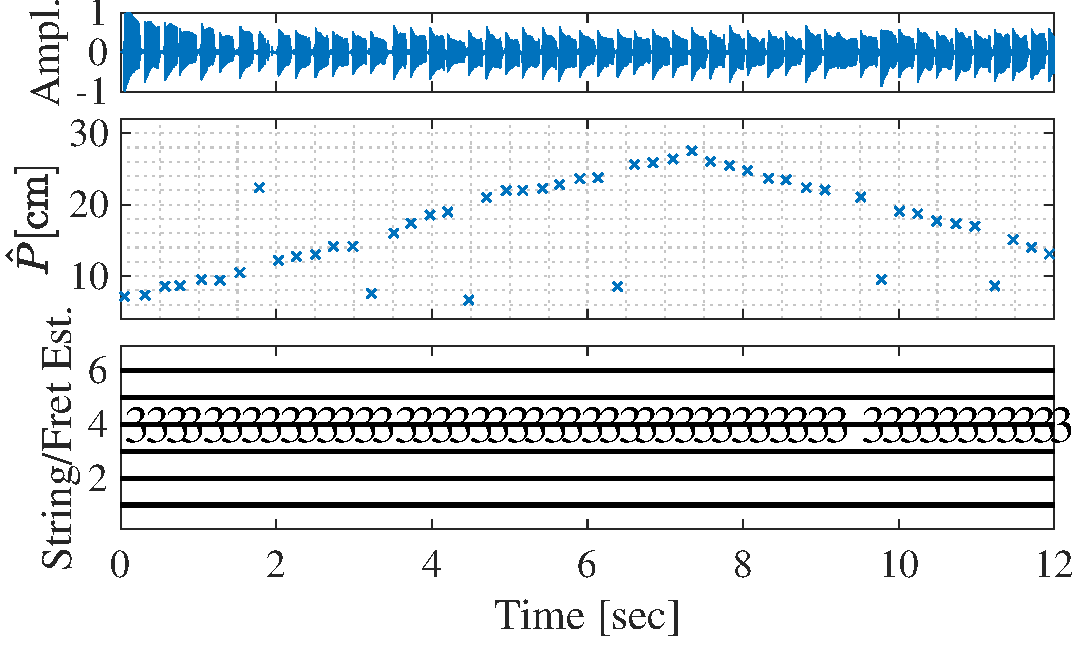
\includegraphics[width=.86\linewidth]{img/tablature_constant_note8}\vspace{-2mm}
   \caption{String, fret and plucking position estimates with moving plucking position and fixed string and fret for electric guitar.}
   \label{fig:pluck_position_fixed_tabs} 
% \end{subfigure}
% \vspace{4mm}
% \begin{subfigure}
%   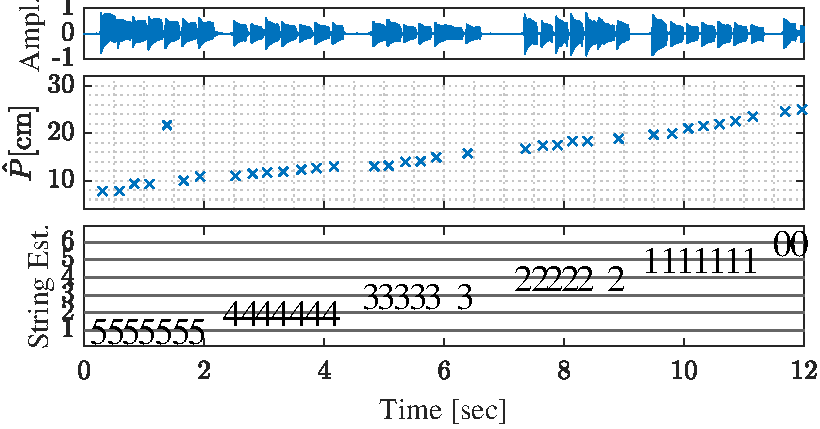
\includegraphics[width=.95\linewidth]{img/tablature_constant_note25_LSD}\vspace{-2mm}
%   \caption{String, fret and plucking position estimates with moving plucking position and moving string and fret for electric guitar.}
%   \label{fig:pluck_position_varied_tabs}
% \end{subfigure}
\end{figure}
%
\section{Conclusion}
Maybe something along the lines of:\\
Now that we have included plucking position to calculate the initial displacement $\delta$ we might be able to also estimate this. 
%
% -------------------------------------------------------------------------
% Either list references using the bibliography style file IEEEtran.bst
\bibliographystyle{IEEEtran}
\bibliography{myabbr,refs17,refs}
%
% or list them by yourself
% \begin{thebibliography}{9}
% 
% \bibitem{waspaa17web}
%   \url{http://www.waspaa.com}.
%
% \bibitem{IEEEPDFSpec}
%   {PDF} specification for {IEEE} {X}plore$^{\textregistered}$,
%   \url{http://www.ieee.org/portal/cms_docs/pubs/confstandards/pdfs/IEEE-PDF-SpecV401.pdf}.
%
% \bibitem{PDFOpenSourceTools}
%   Creating high resolution {PDF} files for book production with 
%   open source tools, 
%   \url{http://www.grassbook.org/neteler/highres_pdf.html}.
%
% \bibitem{eWilliams1999}
% E. Williams, \emph{Fourier Acoustics: Sound Radiation and Nearfield Acoustic
%   Holography}. London, UK: Academic Press, 1999.
% 
% \bibitem{ieeecopyright}
%   \url{http://www.ieee.org/web/publications/rights/copyrightmain.html}.
%
% \bibitem{cJones2003}
% C. Jones, A. Smith, and E. Roberts, ``A sample paper in conference
%   proceedings,'' in \emph{Proc. IEEE ICASSP}, vol. II, 2003, pp. 803--806.
% 
% \bibitem{aSmith2000}
% A. Smith, C. Jones, and E. Roberts, ``A sample paper in journals,'' 
%   \emph{IEEE Trans. Signal Process.}, vol. 62, pp. 291--294, Jan. 2000.
% 
% \end{thebibliography}


\end{sloppy}
\end{document}
